%
% transport.tex
%
% (c) 2021 Prof Dr Andreas Müller, OST Ostschweizer Fachhochschule
%
\documentclass[tikz]{standalone}
\usepackage{times}
\usepackage{amsmath}
\usepackage{txfonts}
\usepackage[utf8]{inputenc}
\usepackage{graphics}
\usetikzlibrary{arrows,intersections,math,calc}
\definecolor{vektora}{rgb}{0.2,0.8,0.2}
\definecolor{vektorb}{rgb}{0.2,0.6,1.0}
\definecolor{rot}{rgb}{1,0.4,0.4}
\usepackage{ifthen}
\begin{document}

\newboolean{showgrid}
\setboolean{showgrid}{false}
\def\breite{7}
\def\hoehe{4}

\begin{tikzpicture}[>=latex,thick]

% Povray Bild
\node at (0,0) {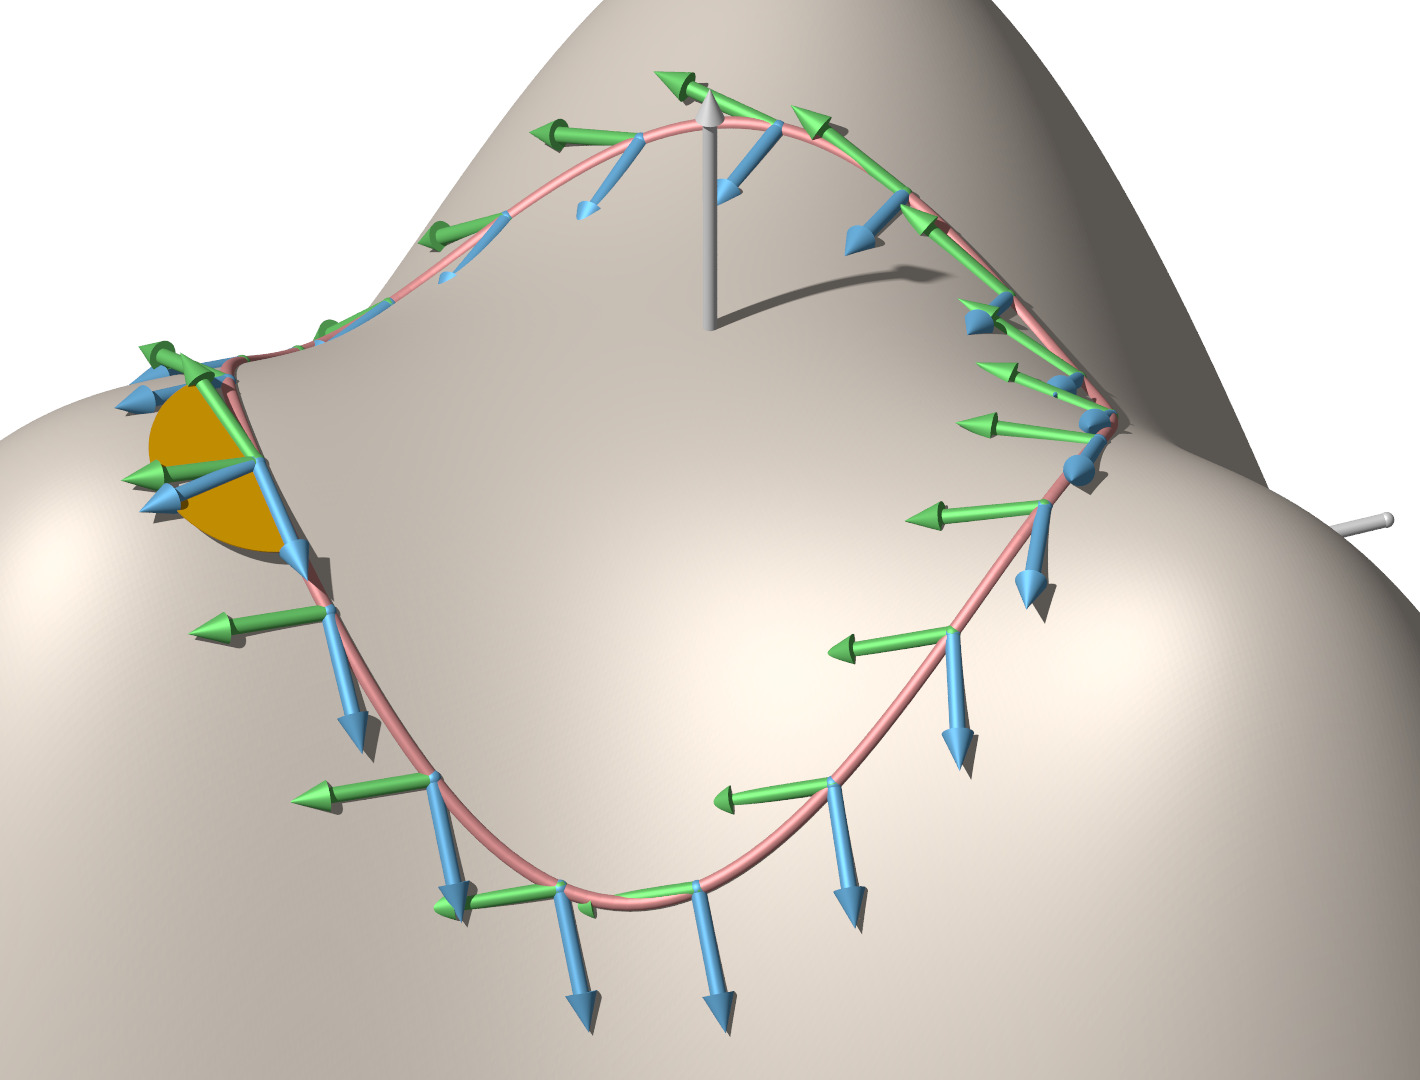
\includegraphics[width=10.5cm]{transport.jpg}};

% Gitter
\ifthenelse{\boolean{showgrid}}{
\draw[step=0.1,line width=0.1pt] (-\breite,-\hoehe) grid (\breite, \hoehe);
\draw[step=0.5,line width=0.4pt] (-\breite,-\hoehe) grid (\breite, \hoehe);
\draw                            (-\breite,-\hoehe) grid (\breite, \hoehe);
\fill (0,0) circle[radius=0.05];
}{}

\node at (-3.08,0.75) {$P$};
\coordinate (P1) at (-4.58,0.5);
\coordinate (P2) at (-2.66,-0.16);
\fill[color=black,opacity=0.4] ($(P1)+(-0.2,-0.2)$) rectangle ++(0.4,0.4);
\node[color=vektora] at (P1) {$\vec{v}_1$};
\fill[color=black,opacity=0.4] ($(P2)+(-0.2,-0.2)$) rectangle ++(0.4,0.4);
\node[color=vektorb] at (P2) {$\vec{v}_2$};

\node[color=white] at (-3.5,0.25) {$\alpha$};
\node[color=white] at (-3.83,0.75) {$\alpha$};
\node[color=rot] at (-1.3,-1.9) {$\gamma(t)$};

\end{tikzpicture}

\end{document}

